\documentclass[letterpaper,11pt,notitlepage]{article}
% define the title
\usepackage{amsmath}
\usepackage{fixltx2e}
\usepackage{graphicx}
\usepackage[labelformat=empty]{caption}
\usepackage{subcaption}
\usepackage{listings}
\usepackage{color}
\usepackage{relsize}
\usepackage{wrapfig}
\usepackage{fontspec}
\usepackage{hyperref}
\usepackage{hanging}
\usepackage{textcomp,    % for \textlangle and \textrangle macros
            xspace}
\newcommand\la{\textlangle}  % set up short-form macros
\newcommand\ra{\textrangle\xspace}
\newcommand\rans{\textrangle}
\lstset{
  language={matlab},
  basicstyle=\ttfamily\smaller\relax,	
  tabsize=4,                              % Default tab size
  % showspaces=false,                       % Dont make spaces visible
  showtabs=false,                         % Dont make tabls visible
  columns=flexible,                       % Column formatc
  commentstyle=\color{mygreen}\textit,           % comment style
  extendedchars=true,              % lets you use non-ASCII characters; for 8-bits encodings only, does not work with UTF-8
  numbers=left,                    % where to put the line-numbers; possible values are (none, left, right)
  numbersep=8pt,                   % how far the line-numbers are from the code
  numberstyle=\tiny\color{mygray}, % the style that is used for the line-numbers
  stepnumber=1,
  xleftmargin=2cm,
  % backgroundcolor=\color{light-gray},
  breaklines=true,
  keywordstyle=\color{mynavy}
}
\hypersetup{colorlinks=true,linkcolor=blue}
\renewcommand*{\UrlFont}{\ttfamily\smaller\relax}

% \addtolength{\oddsidemargin}{0.5in}
% \addtolength{\evensidemargin}{0.5in}
% \addtolength{\textwidth}{-1in}
\addtolength{\topmargin}{-1in}
\addtolength{\textheight}{1.75in}
\setlength\parindent{24pt}

\definecolor{mygreen}{rgb}{0.1020,0.5961,0.3137}
\definecolor{mygray}{rgb}{0.5,0.5,0.5}
\definecolor{light-gray}{rgb}{0.8,0.8,0.8}
\definecolor{mynavy}{rgb}{0.1922,0.2118,0.5843}

\begin{document}

\begin{center}
	Homework 4 - LEARNABILITY\\
	2015 Spring, Machine Learning\\
	Choong-Wan Woo\\
	\today\\
\end{center}

\hspace*{-1cm}\textbf{Problem 2.3.}  \rule{10.5cm}{0.4pt}\\
\noindent\textit{Concentric circles.}\\

\indent With concentric circles as concepts, we can define one annulus error area, \textit{E} (see \textbf{Figure 1}), that has the probability of falling in this region, $\epsilon$. The annulus area, \textit{E}, can be defined as $E = \{(x,y):e^2\le x^2+y^2 \le r^2\}$, with $e = \inf\{e:\Pr[\pi(r^2-e^2)]\ge \epsilon\}$\\
\indent By contraposition, if $R(\text{R}_S)>\epsilon$ (here, $R(\text{R}_S)$ denotes \textit{the expected error of} $\text{R}_S$), then $\text{R}_S$ must miss the error region \textit{E}. As a result, we can write
\begin{align*}
\Pr [R(\text{R}_S)>\epsilon] &\le \Pr[\{\text{R}_S\cap E =\emptyset\}]\\
&\le(1-\epsilon)^m\\
&\le e^{-\epsilon m}
\end{align*}
\noindent For any $\delta >0$, to ensure that $\Pr[R(\text{R}_S) > \epsilon] \le \delta$, we can impose
\[e^{-\epsilon m} \le \delta\]
If we solve this in terms of \textit{m}, we get
\[m \ge \frac{1}{\epsilon}\log \frac{1}{\delta}\]
\noindent Thus, for any $\epsilon >0, \delta>0$, if the sample size \textit{m} is greater than $\frac{1}{\epsilon}\log \frac{1}{\delta}$, then $\Pr[R(\text{R}_S) > \epsilon] \le \delta$. Therefore, this class can be $(\epsilon,\delta)$-PAC-learnable from training data size $m \ge \frac{1}{\epsilon}\log \frac{1}{\delta}$

\begin{figure}[ht!]
	\centering
	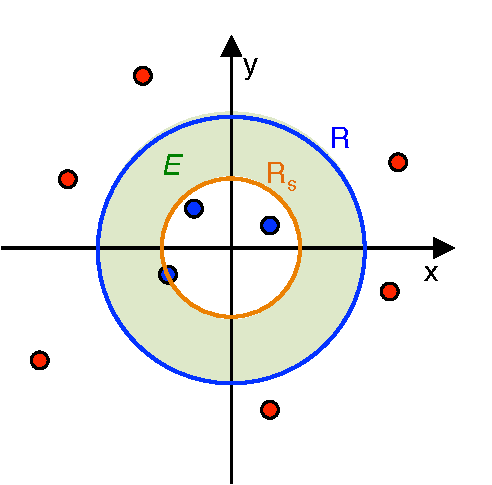
\includegraphics[width=6cm]{Figure1}
	\captionsetup{width=.8\textwidth}
	\caption{\textbf{Figure 1.} Illustration of the concentric circle case.} 
\end{figure}

\hspace*{-1cm}\textbf{Problem 2.4.}  \rule{10.5cm}{0.4pt}\\
\noindent\textit{Non-concentric circles. Can you tell Gertrude if her approach works?}\\

\indent Gertrude's approach will not work because her approach relies on wrong assumptions. Most importantly, with non-concentric circles, false positive errors can be made outside of a target concept, R, as demonstrated in \textbf{Figure 2}. Therefore, drawing three regions, $r_1, r_2, r_3,$ inside R and defining the regions in terms of $\epsilon$ is not useful, and certainly, those three regions, $r_1, r_2, r_3,$ do not have the equal probabilities of $\epsilon$/3.\\
\indent In addition, we can think of a counterexample of Gertrude's approach. As \textbf{Figure 2} shows, even though training data do not miss $r_1, r_2, r_3$ regions, it can still make the generalization error. Thus the equation from her approach 
$\Pr[R(\text{R}_S)>\epsilon]\le \Pr[\bigcup^{3}_{i=1}\{\text{R}_S \bigcap r_i=\emptyset\}]$, which is similar to the equation 2.5 of the textbook, should be wrong in this non-concentric circle case. 

\begin{figure}[ht!]
	\centering
	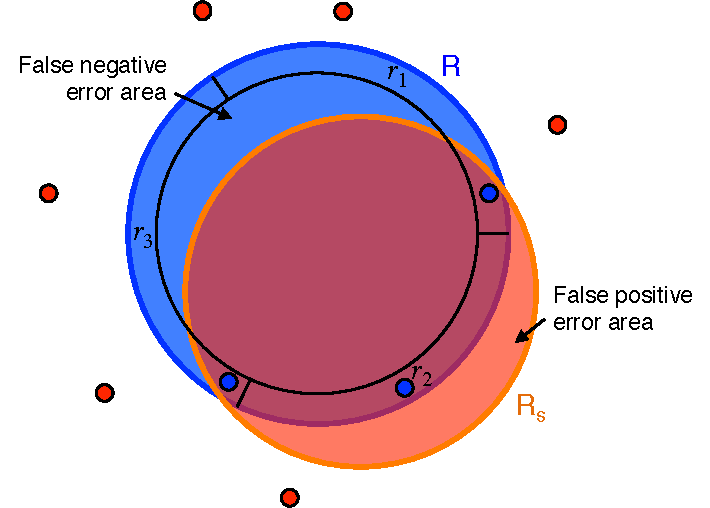
\includegraphics[width=7.5cm]{Figure2}
	\captionsetup{width=.8\textwidth}
	\caption{\textbf{Figure 2.} Illustration of the non-concentric circle case.} 
\end{figure}

\hspace*{-1cm}\textbf{Problem 2.6.}  \rule{10.5cm}{0.4pt}\\
\noindent\textit{Learning in the presence of noise-rectangles.}\\\\

\noindent (a) The probability that $\text{R}^\prime$ misses a region $r_j$ equals the sum of 1) the probability that 
no data in $\text{R}^\prime$ fall on a region $r_j$ and 2) the probability that the positive training point that fall on a region $r_j$ is flipped to negative with probability $\eta^\prime$. 
\begin{align*}
\Pr[\text{R}^\prime \text{ misses }r_j] &= \Pr[\{\text{R}^\prime \cap r_j =\emptyset\}] + \eta^\prime\Pr[\{\text{R}^\prime \cap r_j \neq\emptyset\}]\\
&= 1-\frac{\epsilon}{4} + \eta^\prime\times\frac{\epsilon}{4}\\
&= 1+\frac{(\eta^\prime-1)\epsilon}{4}\\
\end{align*}

\noindent (b) The upper bound on $\Pr[R(\text{R}^\prime)>\epsilon]$ can be derived as follows:
\begin{align*}
\Pr[R(\text{R}^\prime)>\epsilon] &\le \Pr_{S\sim D^m}[\bigcup^{4}_{i=1}\{\text{R}^\prime \text{ misses }r_j\}]\\
&\le \sum^{4}_{i=1} \Pr_{S\sim D^m}[\{\text{R}^\prime \text{ misses }r_j\}]\\
&\le 4(1+\frac{(\eta^\prime-1)\epsilon}{4})^m\\
&\le 4e^{(\eta^\prime-1)m\epsilon/4}\\
\end{align*}

\indent For any $\delta >0$, to ensure that $\Pr[R(\text{R}^\prime)>\epsilon] \le \delta$, we can impose
\[4e^{(\eta^\prime-1)m\epsilon/4} \le \delta\]
\indent, solving for \textit{m}:
\[m\ge\frac{4}{(1-\eta^\prime)\epsilon}\ln\frac{4}{\delta}\]












\end{document}